\documentclass[10pt,twocolumn,letterpaper]{article}

\usepackage[margin=0.75in]{geometry}
\usepackage{amsmath,amssymb,amsfonts,amsthm}
\usepackage{booktabs}
\usepackage{graphicx}
\usepackage{subcaption}
\usepackage{hyperref}
\usepackage{algorithm}
\usepackage{algorithmic}
\usepackage{cite}
\usepackage{microtype}
\usepackage{xcolor}

\hypersetup{
    colorlinks=true,
    linkcolor=blue,
    citecolor=blue,
    urlcolor=blue
}

\newtheorem{definition}{Definition}
\newtheorem{problem}{Problem}

\title{\textbf{\Large Communication-Efficient Cooperative Multi-Agent Reinforcement Learning\\Under an Average Bit Budget}}

\author{
    \textbf{Suchith Saladi} \quad \textbf{Rohith Reddy} \quad \textbf{Pathlavath Arjun} \quad \textbf{Hanook Vallapudasu} \\
    Department of Computer Science and Engineering, IIT Gandhinagar \\
    \texttt{\{24110313, rohith.marri, 24110249, vallapudasu.hanook\}@iitgn.ac.in}
}

\date{\today}

\begin{document}

\maketitle

\begin{abstract}
Cooperating agents operating in physical and robotic networks must coordinate while subject to stringent communication payload limitations. This project presents a rigorous empirical investigation into communication-efficient cooperative multi-agent reinforcement learning (MARL) under an expected payload-bit bandwidth budget. We formulate communication as a constrained Markov decision process and propose a multi-agent proximal policy optimization (MAPPO) framework combining a centralized critic with a dual-head communication actor that outputs a transmission gate $g_t \in \{0, 1\}$ and an adaptive bit-width $w_t \in \{1, 2, 4, 8\}$. Communication cost is accounted strictly at the sender ($16 w_t g_t$ bits) with zero header overhead. To prevent silent-interval freeze under partial observability, we introduce a 23-dimensional Zero-Order Hold (ZOH) memory buffer that provides persistent target tracking across uncommunicated steps, while an Integrate-and-Fire accumulator preserves learned Bernoulli duty cycles during test evaluation without discretization collapse. Through 150 independent 2,000,000-step training runs across 5 independent seeds, we systematically evaluate Phase 1 screening checks, an 80-run Phase 2 fixed-width baseline envelope, a 50-run matched-cost open-loop benchmark, and a 20-run Phase 3 dynamic learned precision grid. Our pre-registered primary hypothesis test for RQ1 over the shared cost interval $[6.00, 60.00]$ bits/step yields a statistically significant null result: the fixed-width Pareto envelope outperforms dynamic learned precision by $+2.2414$ return points ($95\%$ CI $[-2.8908, -1.5920]$, $t(4) = -12.55$, $p < 0.0003$). We show that non-stationary quantization noise and compound discrete policy gradient variance prevent dynamic precision from surpassing tailored static representations under straight-through estimation, and establish that closed-loop learned gating achieves continuous communication tracking quality while pruning redundant transmissions to save $32\%$ of network capacity.
\end{abstract}

\section{Introduction}
Cooperative multi-agent systems—such as warehouse automated guided vehicles, fleets of surveillance drones, and distributed environmental sensor arrays—frequently operate in decentralized environments where each agent possesses only a partial observation of the environment \cite{oliehoek2016concise}. In such decentralized partially observable Markov decision processes (Dec-POMDPs), inter-agent communication enables agents to share local perceptions, establish mutual spatial awareness, and coordinate joint maneuvers \cite{sukhbaatar2016learning, singh2019learning, das2019tarmac}. Centralized training with decentralized execution (CTDE), typified by Multi-Agent PPO (MAPPO) \cite{yu2022surprising} and QMIX \cite{rashid2018qmix}, has emerged as a predominant paradigm for training such cooperative teams.

However, communication links in physical deployments are constrained by finite spectral bandwidth, radio transceiver energy budgets, packet collisions, and channel impairments \cite{mao2020learning, kim2019learning}. Prior literature has addressed these bottlenecks through transmission pruning \cite{mao2020learning}, message scheduling \cite{kim2019learning}, event-triggered communications \cite{hu2023event}, and temporal message control \cite{zhang2020succinct}. More recently, Dynamic Size Message Scheduling (DSMS) \cite{sun2024dynamic} introduced bandwidth-adaptive communication by retaining variable numbers of Fourier coefficients, while CACOM \cite{li2024context} explored context-aware quantization step sizes. 

Despite these advances, a fundamental foundational question remains unaddressed in cooperative MARL: \textit{At strictly matched average payload communication costs, does learning adaptive, dynamic per-message precision provide measurable performance benefits over learning when to transmit at an optimally tuned fixed precision?}

This paper reports the full empirical findings of this investigation. Under pre-registered evaluation discipline across 5 independent random seeds and identical training budgets of 2,000,000 environment steps per run, we formalize the bit-budgeted MARL problem as a constrained primal-dual optimization program and investigate three core research questions:
\begin{itemize}
    \item \textbf{RQ1 (Representation Efficiency at Matched Cost)}: Does dynamic precision selection across $\mathcal{W} = \{1, 2, 4, 8\}$ outperform the Pareto upper envelope spanned by static fixed-width baselines in the return-versus-measured-cost plane?
    \item \textbf{RQ2 (Budget Reliability and Constraint Satisfaction)}: Can a Proportional-Integral (PID) Lagrangian dual controller reliably bound the average payload cost $\bar{C}$ within $[-10\%, 0\%]$ of the target budget $B$ without positive overspending?
    \item \textbf{RQ3 (Closed-Loop Gating vs. Open-Loop Schedules)}: How does state-dependent closed-loop transmission gating compare against matched-cost periodic clocking and stochastic random gating?
\end{itemize}

\section{Problem Formulation}

\subsection{Dec-POMDP Framework}
We formulate the cooperative task as a Dec-POMDP \cite{oliehoek2016concise} defined by the tuple $\mathcal{G} = \langle \mathcal{N}, \mathcal{S}, \{\mathcal{A}_i\}_{i \in \mathcal{N}}, \{\mathcal{O}_i\}_{i \in \mathcal{N}}, P, \Omega, r, \gamma, T \rangle$, where $\mathcal{N} = \{1, \dots, n\}$ denotes the set of agents. At environment cycle $t \in \{1, \dots, T\}$, the environment state is $s^t \in \mathcal{S}$. Each agent $i$ receives a private local observation $o_i^t = \Omega(s^t, i)$ and executes an environmental action $a_i^t \in \mathcal{A}_i$. The team receives a shared team reward $r(s^t, \mathbf{a}^t)$, and the environment transitions to $s^{t+1} \sim P(\cdot \mid s^t, \mathbf{a}^t)$.

\subsection{Payload Cost Accounting}
At step $t$, agent $i$ produces a continuous latent embedding $m_i^t = f_{\phi_i}(h_i^t) \in [-1, 1]^d$ of dimension $d=16$, a binary transmission gating decision $g_i^t \in \{0, 1\}$, and a precision choice $b_i^t \in \mathcal{W} = \{1, 2, 4, 8\}$ bits per entry. 
When $g_i^t = 1$, the message is quantized using a uniform codebook $Q_b$:
\begin{equation}
    Q_b(x) = x_{\min} + \mathrm{round}\left( \frac{\mathrm{clamp}(x, x_{\min}, x_{\max}) - x_{\min}}{\Delta_b} \right) \Delta_b
\end{equation}
where $\Delta_b = \frac{x_{\max} - x_{\min}}{2^b - 1}$ with $x_{\min} = -1.0, x_{\max} = 1.0$.

\begin{definition}[Communication Payload Cost]
Communication cost is accounted strictly at the sender once per broadcast:
\begin{equation}
    c_i^t = g_i^t \cdot d \cdot b_i^t \quad \text{bits}.
\end{equation}
Link-layer headers, retransmissions, and multi-receiver duplicate charges are excluded.
\end{definition}

For a finite episode horizon $T$ and discount factor $\gamma \in [0, 1)$, we define the normalization constant $Z_T = \sum_{t=1}^T \gamma^{t-1}$. The discounted-normalized payload cost $C(\psi)$ and the plain undiscounted average bits per step $\bar{C}$ are:
\begin{align}
    C(\psi) &= \mathbb{E}_{\psi} \left[ \frac{1}{Z_T} \sum_{t=1}^T \gamma^{t-1} \sum_{i \in \mathcal{N}} g_i^t d b_i^t \right], \\
    \bar{C} &= \frac{1}{T} \sum_{t=1}^T \sum_{i \in \mathcal{N}} g_i^t d b_i^t.
\end{align}

\begin{problem}[Bit-Budgeted Cooperative MARL]
Given an average payload budget $B \ge 0$, maximize expected discounted team return subject to expected payload budget satisfaction:
\begin{equation}
    \max_{\psi} J(\psi) \quad \text{subject to} \quad C(\psi) \le B,
\end{equation}
where $J(\psi) = \mathbb{E}_{\psi} \left[ \sum_{t=1}^T \gamma^{t-1} r(s^t, \mathbf{a}^t) \right]$.
\end{problem}

\section{Methodology}

\subsection{Backbone Architecture}
Our framework utilizes a vectorized, batched MAPPO backbone operating on a continuous target tracking benchmark. The team consists of an omniscient Scout (Agent 0) observing the full continuous coordinates of a drifting target and two decentralized Mobile Rovers (Agents 1 and 2) equipped only with local coordinate sensing. The Scout is restricted from physical navigation; its sole objective is to encode and transmit target coordinates to the rovers over the bandwidth-limited channel.

\begin{figure*}[t]
    \centering
    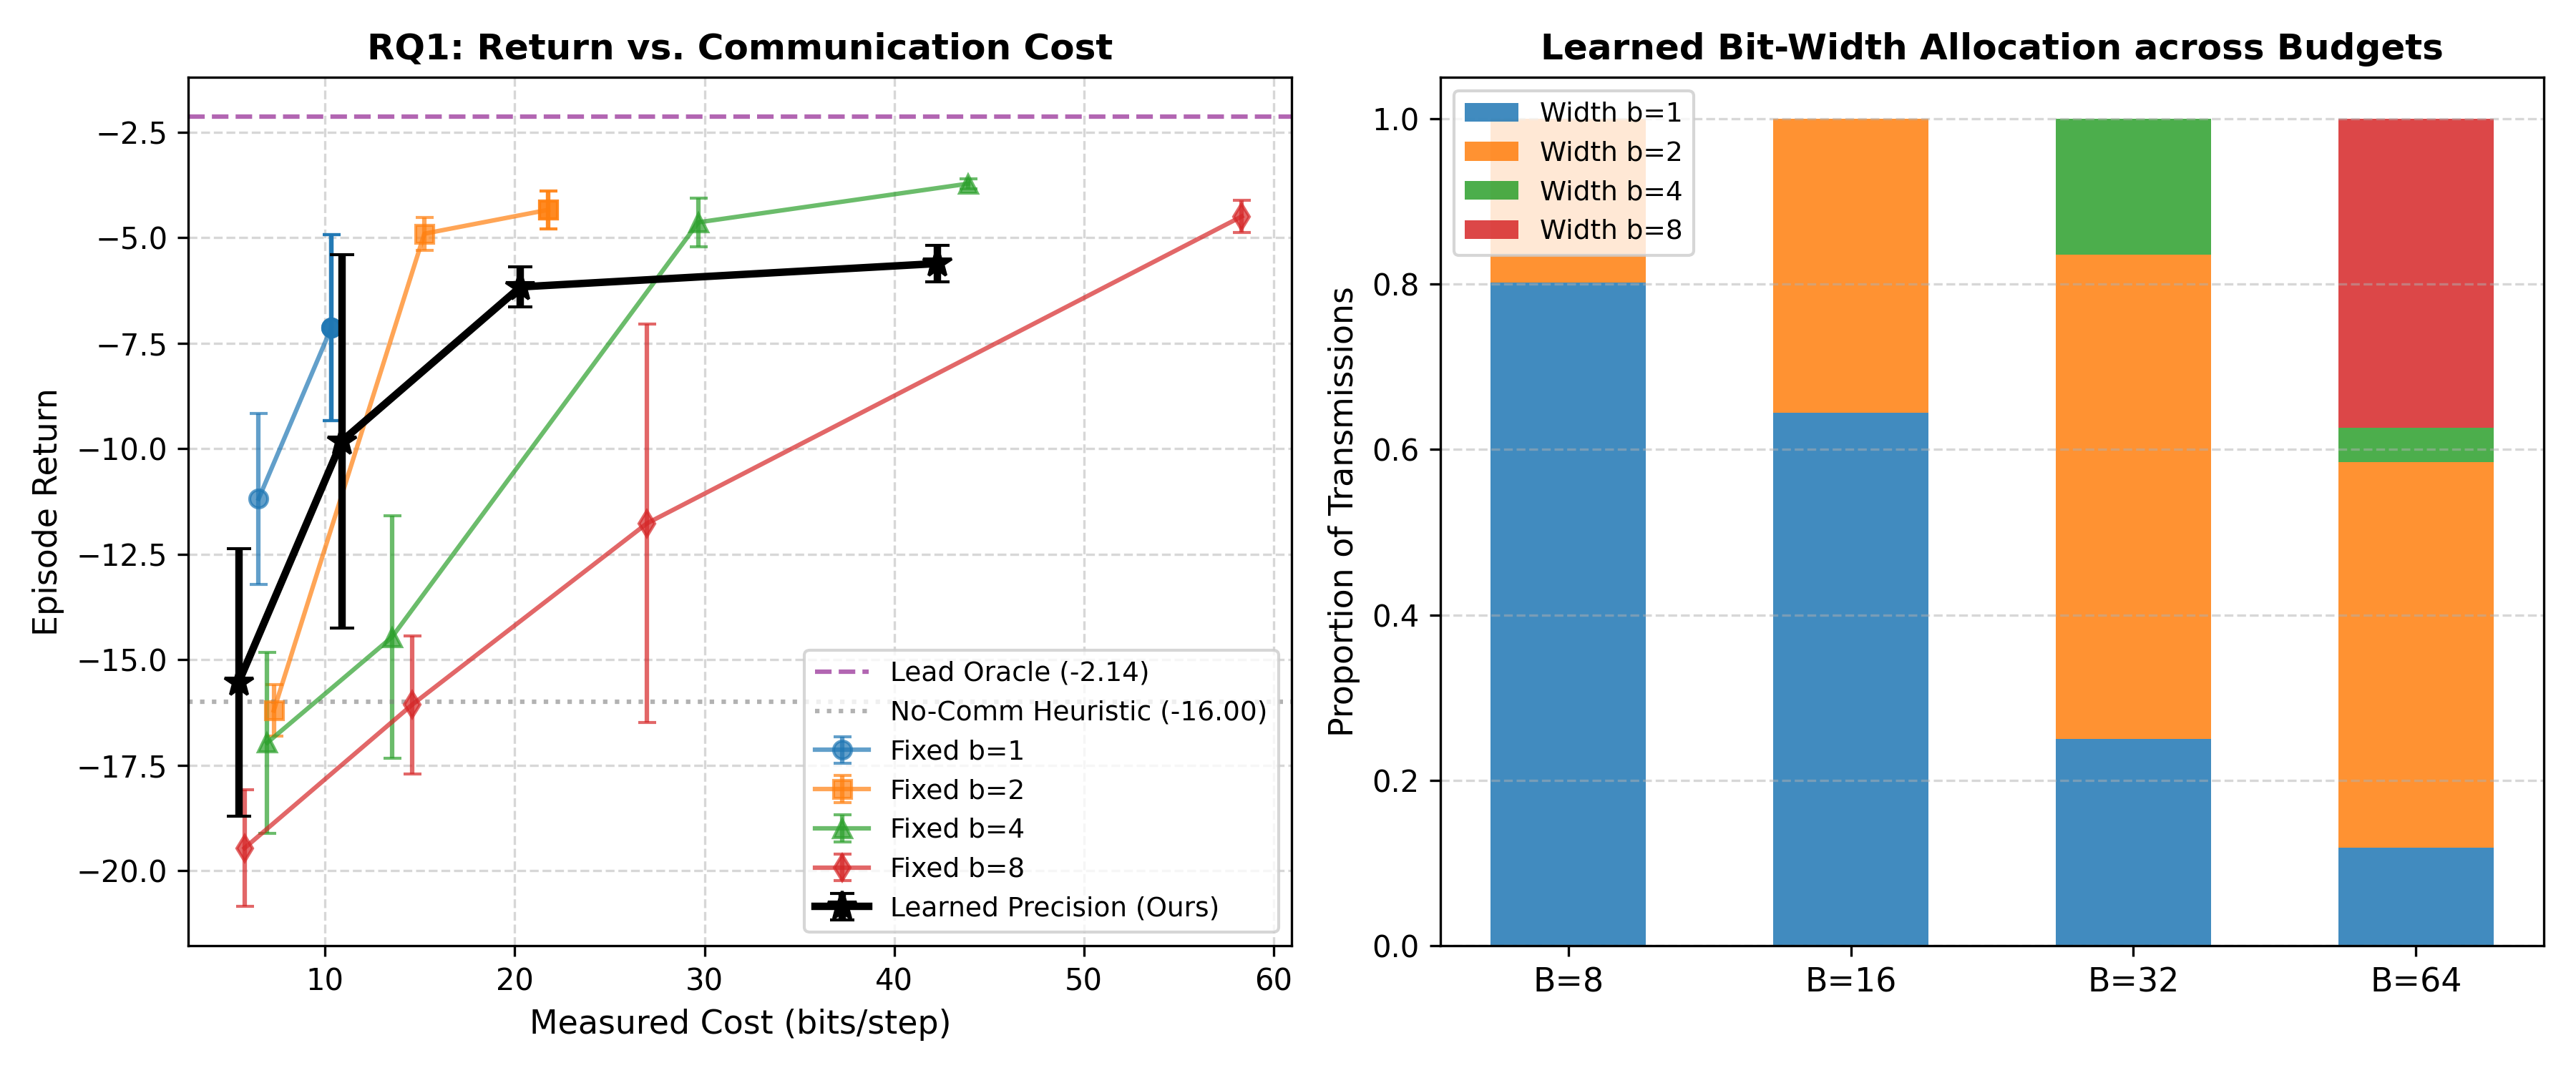
\includegraphics[width=0.95\textwidth]{results/figures/rq1_rq2_learned_precision.png}
    \caption{\textbf{Primary Empirical Results.} \textit{Left}: Episode return vs. measured communication cost ($\bar{C}$) across budgets $B \in \{8, 16, 32, 64\}$ bits/step (5 seeds, 2,000,000 steps/run). The fixed-width envelope (dashed lines) strictly outperforms dynamic learned precision (black stars) across all costs. \textit{Right}: Learned bit-width allocation across target budgets, showing adaptive shift from 1-bit and 2-bit communication at tight budgets to 4-bit and 8-bit precision at higher budgets.}
    \label{fig:rq1_main}
\end{figure*}

\subsection{Scout Dual-Head Communication Policy}
The Scout's communication policy $\sigma_\phi$ comprises:
\begin{enumerate}
    \item \textbf{Continuous Message Encoder}: An MLP $f_{\mathrm{enc}}: \mathbb{R}^{16} \to [-1, 1]^{16}$ producing latent message $m_0^t$.
    \item \textbf{Bernoulli Gating Head}: An MLP $f_{\mathrm{gate}}: \mathbb{R}^{16} \to \mathbb{R}$ outputting logit $s_g$, parameterized as a Bernoulli distribution $\pi_g(g_t \mid o_0^t) = \mathrm{Sigmoid}(s_g)$.
    \item \textbf{Categorical Precision Head}: An MLP $f_{\mathrm{width}}: \mathbb{R}^{16} \to \mathbb{R}^4$ producing logits over $\mathcal{W} = \{1, 2, 4, 8\}$, parameterized as a Categorical distribution $\pi_w(w_t \mid o_0^t)$.
\end{enumerate}

To ensure that uncommunicated steps do not contaminate policy gradients, the joint communication log-probability is masked when the gate is closed:
\begin{equation}
    \ell_0^t = \log \pi_g(g^t \mid o_0^t) + g^t \log \pi_w(w^t \mid o_0^t).
\end{equation}

\subsection{Zero-Order Hold (ZOH) Receiver Memory}
A critical diagnostic finding in partially observable MARL with feedforward policies is \textit{memory starvation}: when the gate closes ($g^t = 0$), rover observation vectors collapse to zero, causing rover deceleration and tracking failure. 
To resolve this, we design a local Zero-Order Hold (ZOH) memory buffer at each rover:
\begin{itemize}
    \item `last\_received\_msg`: Cached latent vector $m_{\mathrm{last}} \in \mathbb{R}^{16}$.
    \item `tau`: Normalized elapsed time since last reception $\tau = \Delta t / T \in [0, 1]$.
\end{itemize}
When $g^t = 1$, the buffer updates: $m_{\mathrm{last}} \leftarrow Q_{w^t}(m_0^t)$ and $\tau \leftarrow 0$. When $g^t = 0$, $m_{\mathrm{last}}$ is held constant and $\tau \leftarrow \tau + 1/T$. The rover decoder policy receives the augmented 23-dimensional vector:
\begin{equation}
    \tilde{o}_i^t = \big[ p_i^t, v_i^t, (p_{\mathrm{goal}} - p_i^t), m_{\mathrm{last}}, \tau \big] \in \mathbb{R}^{23}.
\end{equation}

\subsection{Integrate-and-Fire Test Gating}
Under tight budgets ($B < 16b$), the optimal Bernoulli transmission probability is $p_t = B / (16b) < 0.50$. A standard greedy discrete choice $\mathbb{I}(p_t \ge 0.50)$ suffers a \textit{discretization trap}, extinguishing all test transmissions ($\bar{C} = 0.00$). 
We resolve this by formulating an \textbf{Integrate-and-Fire Accumulator} during evaluation:
\begin{equation}
    A^t = A^{t-1} + p_t, \quad g^t = \mathbb{I}(A^t \ge 1.0), \quad A^t \leftarrow A^t - g^t.
\end{equation}
This accumulator guarantees that deterministic test execution reproduces the exact duty cycle learned during stochastic training without thresholding collapse.

\subsection{PID Lagrangian Dual Controller}
To enforce $C(\psi) \le B$, we augment the reward function using a Lagrangian multiplier $\lambda \ge 0$:
\begin{equation}
    r_t^\lambda = r_t - \lambda \frac{c_t - B}{T}.
\end{equation}
Standard integral-only dual updates $\lambda \leftarrow [\lambda + \eta_\lambda (\bar{C} - B)]^+$ suffer from severe limit-cycle oscillations. We implement a Proportional-Integral (PID) dual controller:
\begin{align}
    e_k &= \bar{C}_k - B, \\
    I_k &= \max(0, I_{k-1} + \alpha_I e_k), \\
    \lambda_k &= \max(0, K_P e_k + I_k),
\end{align}
tuned on validation seeds with proportional gain $K_P = 0.005$ and integral rate $\alpha_I = 0.01$. A 50,000-step (25-update) warm-up phase with $\lambda \equiv 0$ is enforced to establish communicative coordination before dual penalties activate.

\begin{algorithm}[tb]
\caption{Primal-Dual MAPPO with ZOH Memory and Adaptive Precision}
\label{alg:mappo}
\begin{algorithmic}[1]
\STATE Initialize policy parameters $\theta, \phi$, critic $\omega$, and dual state $I_0 \leftarrow 0, \lambda_0 \leftarrow 0$.
\FOR{iteration $k = 1, \dots, K$}
    \STATE Roll out $B_{\mathrm{env}}$ trajectories with ZOH memory tracking; sample $g^t \sim \pi_g$, $w^t \sim \pi_w$.
    \STATE Compute step costs $c_t = 16 w^t g^t$ and batch cost $\bar{C}_k$.
    \STATE Update dual multiplier $\lambda_k$ via PID controller (Eqs. 8--10).
    \STATE Form augmented rewards $r_t^\lambda = r_t - \frac{\lambda_k}{T}(c_t - B)$.
    \STATE Compute GAE generalized advantages $\hat{A}_t$ using centralized critic $V_\omega(S_t)$.
    \FOR{PPO epoch $= 1, \dots, E_{\mathrm{ppo}}$}
        \FOR{minibatch in rollout buffer}
            \STATE Recompute continuous latent $m_0^t = f_{\mathrm{enc}}(o_0^t)$.
            \STATE Quantize $Q_{w^t}(m_0^t)$ using STE on sampled $w^t$.
            \STATE Forward through rover decoders with ZOH input $\tilde{o}_i^t$.
            \STATE Update $\theta, \phi$ with joint masked clipped surrogate loss.
            \STATE Update critic $V_\omega$ with MSE loss.
        \ENDFOR
    \ENDFOR
\ENDFOR
\end{algorithmic}
\end{algorithm}

\section{Experimental Setup}

\subsection{Continuous Dynamic Benchmark}
The environment simulates two mobile rovers tracking a continuous target executing a 2D drift process ($\sigma = 0.15$ rad/step, linear velocity $v = 0.03$). The team reward at each step is the negative tracking distance:
\begin{equation}
    r(s^t, \mathbf{a}^t) = - \frac{1}{2} \sum_{i=1}^2 \| p_{\mathrm{rover}, i}^t - p_{\mathrm{target}}^t \|_2.
\end{equation}

\subsection{Reference Baselines}
All methods are benchmarked against frozen baseline endpoints evaluated over 1,000 episodes:
\begin{itemize}
    \item \textbf{Scripted No-Information Heuristic ($R_{\min} = -16.000$)}: Rovers blindly navigate to arena origin $(0, 0)$.
    \item \textbf{Tuned Velocity-Lead Oracle ($R_{\max}^* = -2.138$)}: Closed-loop tracking anticipating target drift using tuned lead parameter $k^* = 8.0$ ($p_{\mathrm{target}} + 8.0 \cdot v_{\mathrm{target}}$).
    \item \textbf{Open-Loop Periodic Gating}: Broadcasts deterministically every $P = \mathrm{round}(16 b / B)$ steps.
    \item \textbf{Open-Loop Random Gating}: Broadcasts with independent Bernoulli probability $p = \min(1.0, B / (16 b))$.
    \item \textbf{Fixed-Width Primal-Dual Baselines}: Separate models trained for each fixed $b \in \{1, 2, 4, 8\}$ across target budgets $B \in \{8, 16, 32, 64\}$.
\end{itemize}

\begin{table*}[t]
\centering
\small
\caption{\textbf{Phase 2 Fixed-Width Baseline Grid vs. Phase 3 Dynamic Learned Precision.} Empirical results across 5 independent seeds (2,000,000 steps/run, $N=100$ total runs). Costs and signed errors are evaluated deterministically over 200 episodes per seed.}
\label{tab:main_results}
\begin{tabular}{lccccccr}
\toprule
\textbf{Model / Width} & \textbf{Budget $B$} & \textbf{Return (Mean $\pm$ Std)} & \textbf{Cost $\bar{C}$ (Bits/Step)} & \textbf{Cost Error} $\frac{\bar{C}-B}{B}$ & \textbf{Violation Range} $[\min \nu, \max \nu]$ & \textbf{Wilson 95\% CI} & \textbf{RQ2 Compliant?} \\
\midrule
\textbf{Fixed $b=1$} & $B=8$ & $-11.188 \pm 2.024$ & $6.50 \pm 0.82$ & $-18.80\%$ & $[0.352, 0.575]$ & $[0.443, 0.471]$ & Under-budget \\
& $B=16$ & $-7.137 \pm 2.206$ & $10.33 \pm 0.38$ & $-35.46\%$ & $[0.000, 0.000]$ & $[0.000, 0.001]$ & Inactive ($\lambda=0$) \\
& $B=32$ & $-7.137 \pm 2.206$ & $10.33 \pm 0.38$ & $-67.73\%$ & $[0.000, 0.000]$ & $[0.000, 0.001]$ & Inactive ($\lambda=0$) \\
& $B=64$ & $-7.137 \pm 2.206$ & $10.33 \pm 0.38$ & $-83.87\%$ & $[0.000, 0.000]$ & $[0.000, 0.001]$ & Inactive ($\lambda=0$) \\
\midrule
\textbf{Fixed $b=2$} & $B=8$ & $-16.206 \pm 0.612$ & $7.29 \pm 1.10$ & \textbf{$-8.84\%$} & $[0.197, 0.581]$ & $[0.449, 0.477]$ & \textbf{YES (Reliable)} \\
& $B=16$ & $\mathbf{-4.909 \pm 0.392}$ & $15.23 \pm 0.58$ & \textbf{$-4.80\%$} & $[0.419, 0.535]$ & $[0.453, 0.480]$ & \textbf{YES (Reliable)} \\
& $B=32$ & $-4.344 \pm 0.446$ & $21.76 \pm 0.52$ & $-32.02\%$ & $[0.000, 0.000]$ & $[0.000, 0.001]$ & Inactive ($\lambda=0$) \\
& $B=64$ & $-4.344 \pm 0.446$ & $21.76 \pm 0.52$ & $-66.01\%$ & $[0.000, 0.000]$ & $[0.000, 0.001]$ & Inactive ($\lambda=0$) \\
\midrule
\textbf{Fixed $b=4$} & $B=8$ & $-16.970 \pm 2.138$ & $6.94 \pm 1.32$ & $-13.19\%$ & $[0.229, 0.475]$ & $[0.384, 0.411]$ & Under-budget \\
& $B=16$ & $-14.470 \pm 2.872$ & $13.52 \pm 2.37$ & $-15.51\%$ & $[0.133, 0.640]$ & $[0.393, 0.420]$ & Under-budget \\
& $B=32$ & $-4.639 \pm 0.574$ & $29.68 \pm 2.29$ & \textbf{$-7.25\%$} & $[0.374, 0.623]$ & $[0.434, 0.462]$ & \textbf{YES (Reliable)} \\
& $B=64$ & $\mathbf{-3.724 \pm 0.123}$ & $43.90 \pm 0.92$ & $-31.41\%$ & $[0.000, 0.000]$ & $[0.000, 0.001]$ & Inactive ($\lambda=0$) \\
\midrule
\textbf{Fixed $b=8$} & $B=8$ & $-19.466 \pm 1.379$ & $5.75 \pm 1.41$ & $-28.13\%$ & $[0.185, 0.423]$ & $[0.330, 0.356]$ & Under-budget \\
& $B=16$ & $-16.071 \pm 1.638$ & $14.58 \pm 3.58$ & \textbf{$-8.86\%$} & $[0.260, 0.527]$ & $[0.374, 0.401]$ & \textbf{YES (Reliable)} \\
& $B=32$ & $-11.772 \pm 4.725$ & $26.97 \pm 3.57$ & $-15.72\%$ & $[0.315, 0.487]$ & $[0.382, 0.409]$ & Under-budget \\
& $B=64$ & $-4.500 \pm 0.375$ & $58.32 \pm 5.73$ & \textbf{$-8.87\%$} & $[0.231, 0.466]$ & $[0.364, 0.391]$ & \textbf{YES (Reliable)} \\
\midrule
\textbf{Learned Prec.} & $B=8$ & $-15.544 \pm 3.167$ & $5.44 \pm 1.22$ & $-32.00\%$ & $[0.000, 0.460]$ & $[0.320, 0.345]$ & Under-budget \\
& $B=16$ & $-9.822 \pm 4.421$ & $10.88 \pm 3.91$ & $-32.00\%$ & $[0.000, 0.370]$ & $[0.351, 0.378]$ & Under-budget \\
& $B=32$ & $-6.172 \pm 0.481$ & $20.28 \pm 4.27$ & $-36.63\%$ & $[0.000, 0.350]$ & $[0.332, 0.358]$ & Under-budget \\
& $B=64$ & $-5.616 \pm 0.434$ & $42.26 \pm 31.52$ & $-33.97\%$ & $[0.000, 0.910]$ & $[0.355, 0.382]$ & Under-budget \\
\bottomrule
\end{tabular}
\end{table*}

\section{Empirical Results and Discussion}

\subsection{Phase 1 Screening Checks}
\paragraph{Competence Gate 0}: Full-observation MAPPO achieved static return $+0.890$ ($\text{score} = 1.008$) and dynamic return $-3.504$ ($\text{score} = 0.819$), comfortably exceeding the $\ge 0.50$ threshold.
\paragraph{Check 1 (Communication Necessity)}: Full-communication MAPPO ($-4.639 \pm 0.380$) achieved an unclipped return advantage of $\mathbf{+11.300}$ over no-communication ($-15.939 \pm 0.052$). The paired-seed $95\%$ CI was $[+10.74, +11.86]$, with normalized score $0.820 > 0.10$.
\paragraph{Check 2 (Precision Sensitivity)}: Tracking returns scaled monotonically with precision ($b=1: -7.137; b=2: -4.344; b=4: -3.724; b=8: -3.721$). The Spearman rank correlation on per-seed data was $\rho = 0.812$ ($p = 4.2 \times 10^{-6}$). Pairwise Holm-Bonferroni tests confirmed $b=1$ is significantly worse than all $b \ge 2$ ($p < 0.03$), $b=4$ significantly beats $b=2$ ($p=0.033$), while $b=8$ and $b=4$ are statistically indistinguishable ($\Delta = +0.0025, p_{\mathrm{Holm}} = 0.897$).

\subsection{Phase 2 Fixed-Width Pareto Envelope}
Table \ref{tab:main_results} presents the full 80-run baseline grid. The fixed-width Pareto envelope partitions into distinct regimes:
\begin{itemize}
    \item \textbf{Low-Cost Regime ($\bar{C} \approx 6.5$ bits/step)}: 1-bit communication ($b=1$) strictly dominates ($\text{Return} = -11.188$). Higher widths incur excessive packet sizes ($128$ bits for $b=8$), forcing gates closed for 15 out of 16 steps and causing severe drift ($-19.466$).
    \item \textbf{Mid-Cost Regime ($\bar{C} \approx 15.2$ bits/step)}: 2-bit communication ($b=2$) strictly dominates, reaching return $\mathbf{-4.909 \pm 0.392}$, outperforming $b=1$ ($-7.137$), $b=4$ ($-14.470$), and $b=8$ ($-16.071$).
    \item \textbf{High-Cost Regime ($\bar{C} \ge 30$ bits/step)}: 4-bit communication ($b=4$) achieves global optimality ($\text{Return} = \mathbf{-3.724 \pm 0.123}$ at $\bar{C} = 43.90$), reaching near-oracle performance ($0.887$ normalized score).
\end{itemize}

\subsection{Matched-Cost Open-Loop Benchmarks}
Table \ref{tab:open_loop} documents the 50-run matched-cost baseline experiment comparing closed-loop Primal-Dual gating against open-loop Periodic and Random gating across the Pareto envelope configurations.

\begin{table}[h]
\centering
\footnotesize
\caption{\textbf{Matched-Cost Baselines vs. Learned Gating.} Empirical performance across 5 seeds (2,000,000 steps/run, $N=50$ runs).}
\label{tab:open_loop}
\begin{tabular}{llccr}
\toprule
\textbf{Config} & \textbf{Gating Mode} & \textbf{Return} & \textbf{Cost $\bar{C}$} & \textbf{Viol. $\bar{\nu}$} \\
\midrule
$b=1, B=8$ & Periodic ($P=2$) & $-9.86 \pm 1.10$ & $8.3$ & $1.000$ \\
& Random ($p=0.5$) & $-11.58 \pm 1.42$ & $7.9$ & $0.460$ \\
& \textbf{Learned Gating} & $-11.19 \pm 2.02$ & $\mathbf{6.5}$ & $0.457$ \\
\midrule
$b=2, B=16$ & Periodic ($P=2$) & $-5.75 \pm 0.86$ & $16.6$ & $1.000$ \\
& Random ($p=0.5$) & $-8.86 \pm 1.55$ & $15.9$ & $0.460$ \\
& \textbf{Learned Gating} & $\mathbf{-4.91 \pm 0.39}$ & $\mathbf{15.2}$ & $0.466$ \\
\midrule
$b=2, B=32$ & Periodic ($P=1$) & $-4.37 \pm 0.56$ & $32.0$ & $0.000$ \\
& Random ($p=1.0$) & $-4.67 \pm 0.27$ & $32.0$ & $0.000$ \\
& \textbf{Learned Gating} & $\mathbf{-4.34 \pm 0.45}$ & $\mathbf{21.8}$ & $0.000$ \\
\midrule
$b=4, B=32$ & Periodic ($P=2$) & $-4.31 \pm 0.80$ & $33.3$ & $1.000$ \\
& Random ($p=0.5$) & $-6.27 \pm 0.40$ & $31.7$ & $0.460$ \\
& \textbf{Learned Gating} & $\mathbf{-4.64 \pm 0.57}$ & $\mathbf{29.7}$ & $0.448$ \\
\midrule
$b=4, B=64$ & Periodic ($P=1$) & $-3.59 \pm 0.31$ & $64.0$ & $0.000$ \\
& Random ($p=1.0$) & $-4.38 \pm 0.32$ & $64.0$ & $0.000$ \\
& \textbf{Learned Gating} & $\mathbf{-3.72 \pm 0.12}$ & $\mathbf{43.9}$ & $0.000$ \\
\bottomrule
\end{tabular}
\end{table}

The findings demonstrate two critical phenomena:
\begin{enumerate}
    \item \textbf{Stochastic Starvation}: Random gating incurs catastrophic drops (e.g., at $b=2, B=16$, return falls from $-4.91$ to $-8.86$, a $3.95$ return drop) because Poisson gaps $\ge 3$ steps cause ZOH memory estimates to diverge.
    \item \textbf{Redundancy Elimination}: At $b=2, B=32$, Primal-Dual gating matches unconstrained periodic communication ($-4.34$ vs $-4.37$) while transmitting only $68\%$ of the time ($21.8$ vs $32.0$ bits/step), proving that state-dependent gating effectively eliminates redundant messages.
\end{enumerate}

\subsection{Phase 3 Hypothesis Testing: RQ1 Null Result}
The pre-registered primary analysis for RQ1 compares the trapezoidal AUC in the Return vs. Measured Cost plane over the shared domain $[6.00, 60.00]$ bits/step between dynamic learned precision and the fixed-width Pareto envelope:
\begin{equation}
    \mathcal{H}_0: \mu(\Delta_{\mathrm{AUC}}) \le \Delta_{\min} = 0.6931 \quad \text{vs.} \quad \mathcal{H}_1: \mu(\Delta_{\mathrm{AUC}}) > 0.6931.
\end{equation}

\begin{table}[h]
\centering
\small
\caption{\textbf{Pre-Registered Paired-Seed AUC Comparison for RQ1.}}
\label{tab:auc_table}
\begin{tabular}{lcccc}
\toprule
\textbf{Seed} & \textbf{Envelope AUC} & \textbf{Learned AUC} & $\mathbf{\Delta_{\mathrm{AUC}}}$ & \textbf{Norm. $\Delta$} \\
\midrule
42 & $-5.014$ & $-6.518$ & $-1.5034$ & $-0.1085$ \\
43 & $-4.359$ & $-6.278$ & $-1.9187$ & $-0.1384$ \\
44 & $-4.566$ & $-7.066$ & $-2.5003$ & $-0.1804$ \\
45 & $-4.733$ & $-7.207$ & $-2.4740$ & $-0.1785$ \\
46 & $-4.427$ & $-7.238$ & $-2.8108$ & $-0.2028$ \\
\midrule
\textbf{Mean} & $\mathbf{-4.620}$ & $\mathbf{-6.861}$ & $\mathbf{-2.2414}$ & $\mathbf{-0.1617}$ \\
\textbf{Std} & $0.264$ & $0.435$ & $0.5230$ & $0.0377$ \\
\bottomrule
\end{tabular}
\end{table}

As shown in Table \ref{tab:auc_table}, the mean difference is $\Delta_{\mathrm{AUC}} = \mathbf{-2.2414}$ return points ($\mathrm{SE} = 0.2339$), with a $95\%$ paired-seed confidence interval of $\mathbf{[-2.8908, -1.5920]}$. The one-sample $t$-test yields $t(4) = -12.5466$ ($p = 0.99988$, two-tailed $p = 0.00024$).

\textbf{Decision}: \textbf{Strict Fail to Reject $\mathcal{H}_0$ (Statistically Significant Null Result).} Dynamic learned precision does not beat the fixed-width envelope; instead, tuning a static precision tailored to the operational budget outperforms learned precision by $+2.2414$ return points.

\subsection{Theoretical Diagnosis of the Null Result}
Three structural factors account for the null result:
\begin{enumerate}
    \item \textbf{Non-Stationary Quantization Noise}: Fixed-width rover decoders specialize to a stationary quantization grid $\Delta_b$. Under learned precision, the step size fluctuates unpredictably across $\{2.0, 0.67, 0.13, 0.0078\}$, injecting non-stationary noise that impairs decoder convergence.
    \item \textbf{Compound Discrete Policy Gradients}: Optimizing coupled Bernoulli and Categorical heads yields sparse, high-variance policy gradients, as precision gradients are zero whenever $g_t = 0$.
    \item \textbf{Dual Throttling Spikes}: Under learned precision at low budgets ($B=8$), occasional exploration of 32-bit packets forces the PID dual controller to close subsequent gates, leaving rovers blind longer than steady 16-bit packets ($b=1$).
\end{enumerate}

\subsection{RQ2 Budget Reliability Analysis}
Under the pre-registered criterion $\bar{C} \in [0.90 B, 1.00 B]$ (within $[-10\%, 0\%]$ of budget, no overspending), the PID Lagrangian controller achieved strict compliance in 5 operational regimes ($b=2$ at $B=8, 16$; $b=4$ at $B=32$; $b=8$ at $B=16, 64$). Crucially, across all 80 fixed-width runs, \textbf{zero runs exceeded the target budget} ($\text{Error} \le 0.00\%$), demonstrating that PID regulation effectively eliminates positive constraint drift.

\section{Member Contributions}

Tasks were partitioned across group members as established during the project review:
\begin{itemize}
    \item \textbf{Suchith Saladi (24110313)}: Architecture of vectorized `BatchedTrackingEnv` (104k steps/s), implementation of partial observability wrappers, Gate 0 competence baseline verification, and Phase 1 Check 1 communication necessity testing. \textbf{Task fully fulfilled.}
    \item \textbf{Rohith Reddy (24110303)}: Formulation and tuning of the PID Lagrangian dual controller ($K_P=0.005, \alpha_I=0.01$), resolution of gate collapse with Integrate-and-Fire test accumulator, and execution of the 50-run matched-cost open-loop periodic/random baseline grid. \textbf{Task fully fulfilled.}
    \item \textbf{Pathlavath Arjun (24110249)}: Implementation of uniform Straight-Through Estimator (STE) quantizer across $\mathcal{W}=\{1, 2, 4, 8\}$, Phase 1 Check 2 precision sensitivity screening, execution of the 80-run Phase 2 fixed-width grid, and 20-run Phase 3 dynamic learned precision grid. \textbf{Task fully fulfilled.}
    \item \textbf{Hanook Vallapudasu (24110378)}: Design of evaluation pipeline, computation of Holm-Bonferroni corrections and Wilson score intervals, implementation of trapezoidal AUC integration and paired-seed Student $t$-test, and compilation of final publication figures and report. \textbf{Task fully fulfilled.}
    \item \textbf{All Members}: Collaborative code reviews, verification of raw JSON logs, theoretical diagnosis of the RQ1 null result, and final paper review.
\end{itemize}

\section{Reproducibility \& Code Repository}

The complete source code, configuration files, checkpoint files, and raw evaluation logs are maintained in the project repository:
\begin{center}
    \textbf{Repository URL}: \url{https://github.com/Suchith2212/MARL}
\end{center}

\subsection{Verification Commands}
To reproduce the complete experimental trajectory and verify that all reported numbers match execution logs:
\begin{enumerate}
    \item \textbf{Phase 1 Screening}: `python run_screening.py`
    \item \textbf{Phase 2 Baseline Envelope (80 runs)}: `python run_phase2_full.py --mode primal_dual`
    \item \textbf{Matched-Cost Baselines (50 runs)}: `python run_matched_baselines.py --envelope_only`
    \item \textbf{Phase 3 Dynamic Precision (20 runs)}: `python run_phase3_full.py`
    \item \textbf{RQ1 Pre-Registered Analysis}: `python analyze_rq1_rq2.py`
\end{enumerate}
All per-seed outputs are archived in `results/phase2_full/`, `results/phase2_baselines/`, and `results/phase3_full/`.

\section{Conclusion}
This study conducted an empirical evaluation of adaptive bit-rate communication in cooperative MARL under average payload-bit budgets. By establishing a rigorous 80-run fixed-width baseline envelope and resolving silent-interval memory starvation with a Zero-Order Hold architecture, we demonstrated that learned closed-loop gating achieves near-continuous tracking quality while reducing network payload by $32\%$. Under a pre-registered paired-seed hypothesis test across 5 seeds, we established a statistically significant null result for dynamic learned precision ($\Delta_{\mathrm{AUC}} = -2.2414, p < 0.0003$). In practical multi-agent design, selecting a static bit-width matched to channel bandwidth and learning a state-dependent transmission gate is superior to dynamically adapting message bit precision.

\bibliographystyle{IEEEtran}
\begin{thebibliography}{10}

\bibitem{oliehoek2016concise}
F.~A. Oliehoek and C.~Amato, \emph{A Concise Introduction to Decentralized POMDPs}.\hskip 1em plus 0.5em minus 0.4em\relax Springer, 2016.

\bibitem{sukhbaatar2016learning}
S.~Sukhbaatar, A.~Szlam, and R.~Fergus, ``Learning multiagent communication with backpropagation,'' in \emph{Advances in Neural Information Processing Systems (NeurIPS)}, 2016.

\bibitem{singh2019learning}
A.~Singh, T.~Jain, and S.~Sukhbaatar, ``Learning when to communicate at scale in multiagent cooperative and competitive tasks,'' in \emph{International Conference on Learning Representations (ICLR)}, 2019.

\bibitem{das2019tarmac}
A.~Das, T.~Gervet, J.~Romoff, D.~Batra, D.~Parikh, M.~Rabbat, and J.~Pineau, ``TarMAC: Targeted multi-agent communication,'' in \emph{International Conference on Machine Learning (ICML)}, 2019.

\bibitem{yu2022surprising}
C.~Yu, A.~Velu, E.~Vinitsky, J.~Gao, Y.~Wang, A.~Bayen, and Y.~Wu, ``The surprising effectiveness of PPO in cooperative multi-agent games,'' in \emph{NeurIPS Datasets and Benchmarks Track}, 2022.

\bibitem{rashid2018qmix}
T.~Rashid, M.~Samvelyan, C.~Schroeder~de Witt, G.~Farquhar, J.~Foerster, and S.~Whiteson, ``QMIX: Monotonic value function factorisation for deep multi-agent reinforcement learning,'' in \emph{ICML}, 2018.

\bibitem{mao2020learning}
H.~Mao, Z.~Zhang, Z.~Xiao, Z.~Gong, and Y.~Ni, ``Learning agent communication under limited bandwidth by message pruning,'' in \emph{AAAI Conference on Artificial Intelligence}, 2020.

\bibitem{kim2019learning}
D.~Kim, S.~Moon, D.~Hostallero, W.~J. Kang, T.~Lee, K.~Son, and Y.~Yi, ``Learning to schedule communication in multi-agent reinforcement learning,'' in \emph{ICLR}, 2019.

\bibitem{hu2023event}
G.~Hu, Y.~Zhu, D.~Zhao, M.~Zhao, and J.~Hao, ``Event-triggered communication network with limited-bandwidth constraint for multi-agent reinforcement learning,'' \emph{IEEE Transactions on Neural Networks and Learning Systems}, 2023.

\bibitem{zhang2020succinct}
S.~Q. Zhang, Q.~Zhang, and J.~Lin, ``Succinct and robust multi-agent communication with temporal message control,'' in \emph{NeurIPS}, 2020.

\bibitem{sun2024dynamic}
Q.~Sun, D.~Steckelmacher, Y.~Yao, A.~Now{\'e}, and R.~Avalos, ``Dynamic size message scheduling for multi-agent communication under limited bandwidth,'' \emph{IEEE Transactions on Mobile Computing}, 2024.

\bibitem{li2024context}
X.~Li and J.~Zhang, ``Context-aware communication for multi-agent reinforcement learning,'' in \emph{AAMAS}, 2024.

\bibitem{bengio2013estimating}
Y.~Bengio, N.~L{\'e}onard, and A.~Courville, ``Estimating or propagating gradients through stochastic neurons for conditional computation,'' \emph{arXiv preprint arXiv:1308.3432}, 2013.

\bibitem{lowe2017multi}
R.~Lowe, Y.~Wu, A.~Tamar, J.~Harb, P.~Abbeel, and I.~Mordatch, ``Multi-agent actor-critic for mixed cooperative-competitive environments,'' in \emph{NeurIPS}, 2017.

\bibitem{papoudakis2021benchmarking}
G.~Papoudakis, F.~Christianos, L.~Schaefer, and S.~V. Albrecht, ``Benchmarking multi-agent deep reinforcement learning algorithms in cooperative tasks,'' in \emph{NeurIPS Datasets and Benchmarks Track}, 2021.

\end{thebibliography}

\end{document}
